\section{Spoofing}
This section will explore the impact of simulated cyber-spoofing attacks, which were performed by manipulating the previously captured open sky measurement. We triggered different attack conditions starting at $t=100$ s to observe how the receiver handles spatial (and also temporal) anomalies.

\subsection{Position Spoofing near receiver (without delay)}
In this scenario, we simulated a spoofing attack by altering the \texttt{spoof.position} coordinates without injecting any delay. 
When observing the pseudoranges' variation over time, the attack is virtually imperceptible: because the geometric shift induced by the spoofing is relatively small (around 100-150 meters) no obvious step is immediately visible. However, the attack is easily exposed by analyzing the WLS solver, which takes these manipulated measurements and causes an instantaneous jump in latitude, longitude, and altitude. Given that no artificial delay was introduced, the receiver's clock bias remains perfectly continuous and unaffected by the spoofing injection: the algorithm interprets the pseudorange jumps simply as an instantaneous physical translation of the receiver in space, validating the "stealthiness" of a purely geometric spoofing attack.

\begin{figure}[htbp]
    \centering
    %\begin{subfigure}{0.48\columnwidth}
     %   \centering
      %  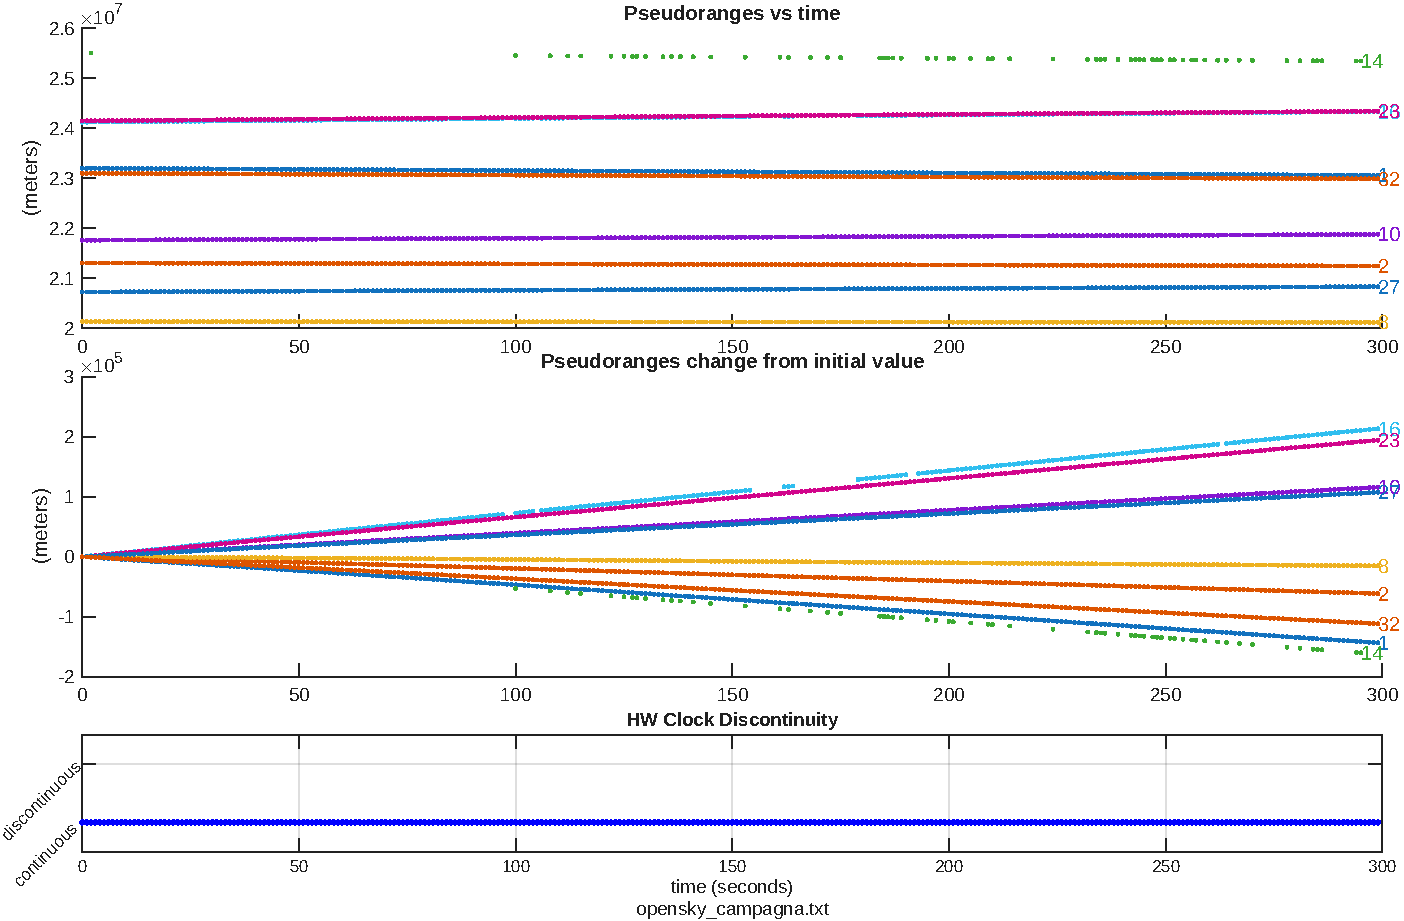
\includegraphics[width=\linewidth]{images/campagna_spoofing_no_delay/Figure_1.pdf}
      %  \caption{Pseudoranges evolution}
       % \label{fig:spoof_far_pr}
    %\end{subfigure}\hfill
    \begin{subfigure}{0.85\columnwidth}
        \centering
        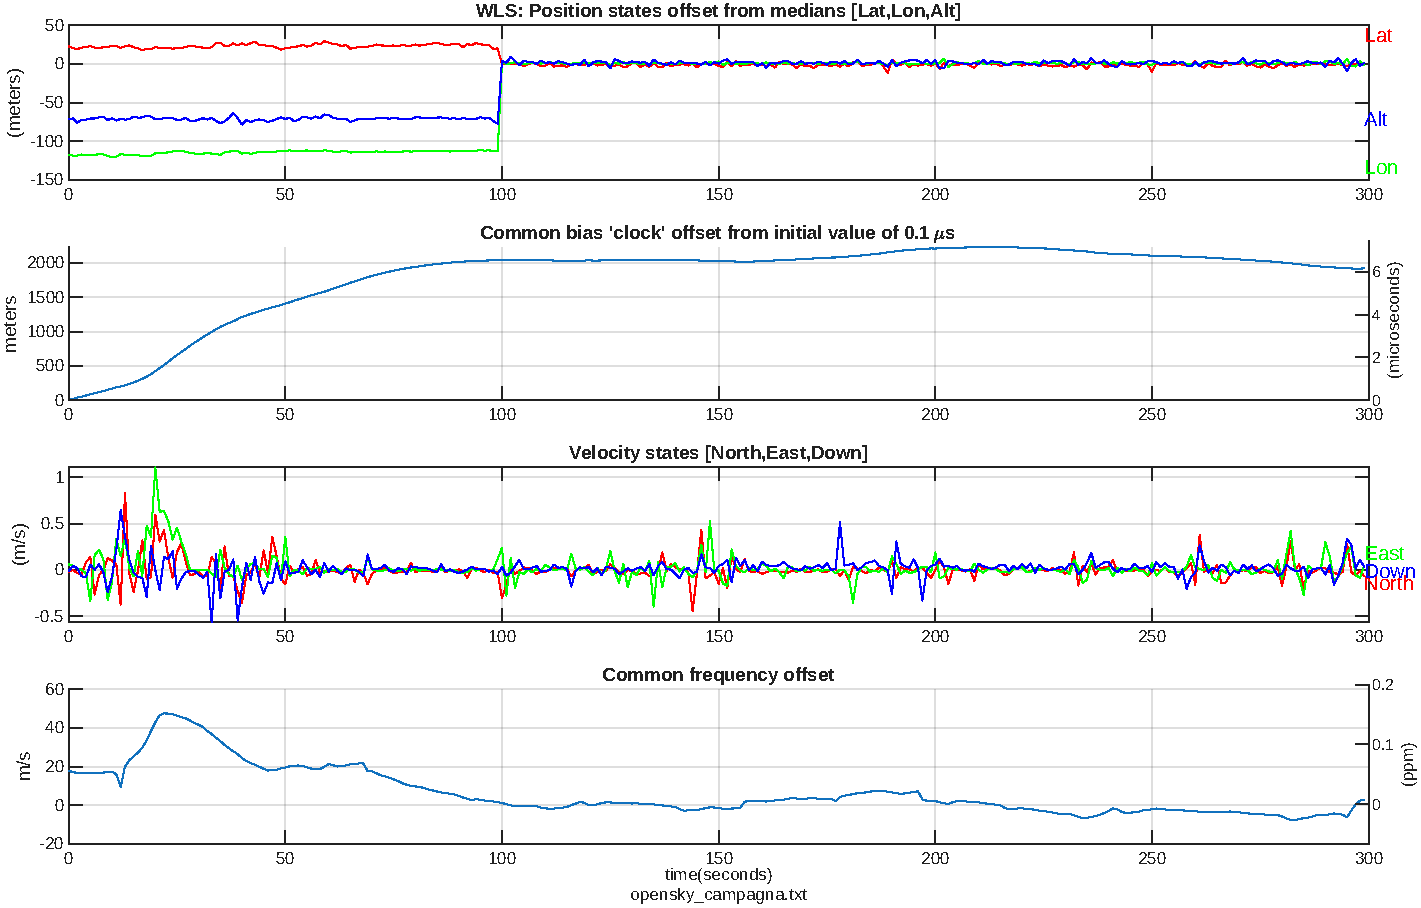
\includegraphics[width=\linewidth]{images/campagna_spoofing_no_delay/Figure_5.pdf}
        \caption{Position states and Clock bias}
        \label{fig:spoof_far_states}
    \end{subfigure}
    \label{fig:spoof_far_results}
\end{figure}

\subsection{Position Spoofing near receiver (with delay)}
In this second scenario, we injected both a false spatial position and a specific \texttt{spoof.delay} at 100 seconds: this new addition creates a massive vertical step across all pseudoranges simultaneously. Because satellite signals travel at the speed of light, even a fractional time delay introduced by the attacker translates into hundreds of kilometers of artificial distance added to every measurement. The WLS solver processes this new measurement and interprets it as a massive receiver clock error. As shown in Figure \ref{fig:spoof_delay_states}, while the spatial coordinates (latitude, longitude, altitude) still snap to the fake location, the clock bias experiences an instant, drastic jump exactly at 100 seconds. This behavior highlights a critical trade-off for an attacker: while introducing a delay might be physically necessary to "capture" the target receiver in a real-world over-the-air attack, it leaves an obvious anomaly in the clock bias domain.

\begin{figure}[htbp]
    \centering
    \begin{subfigure}{0.85\columnwidth}
        \centering
        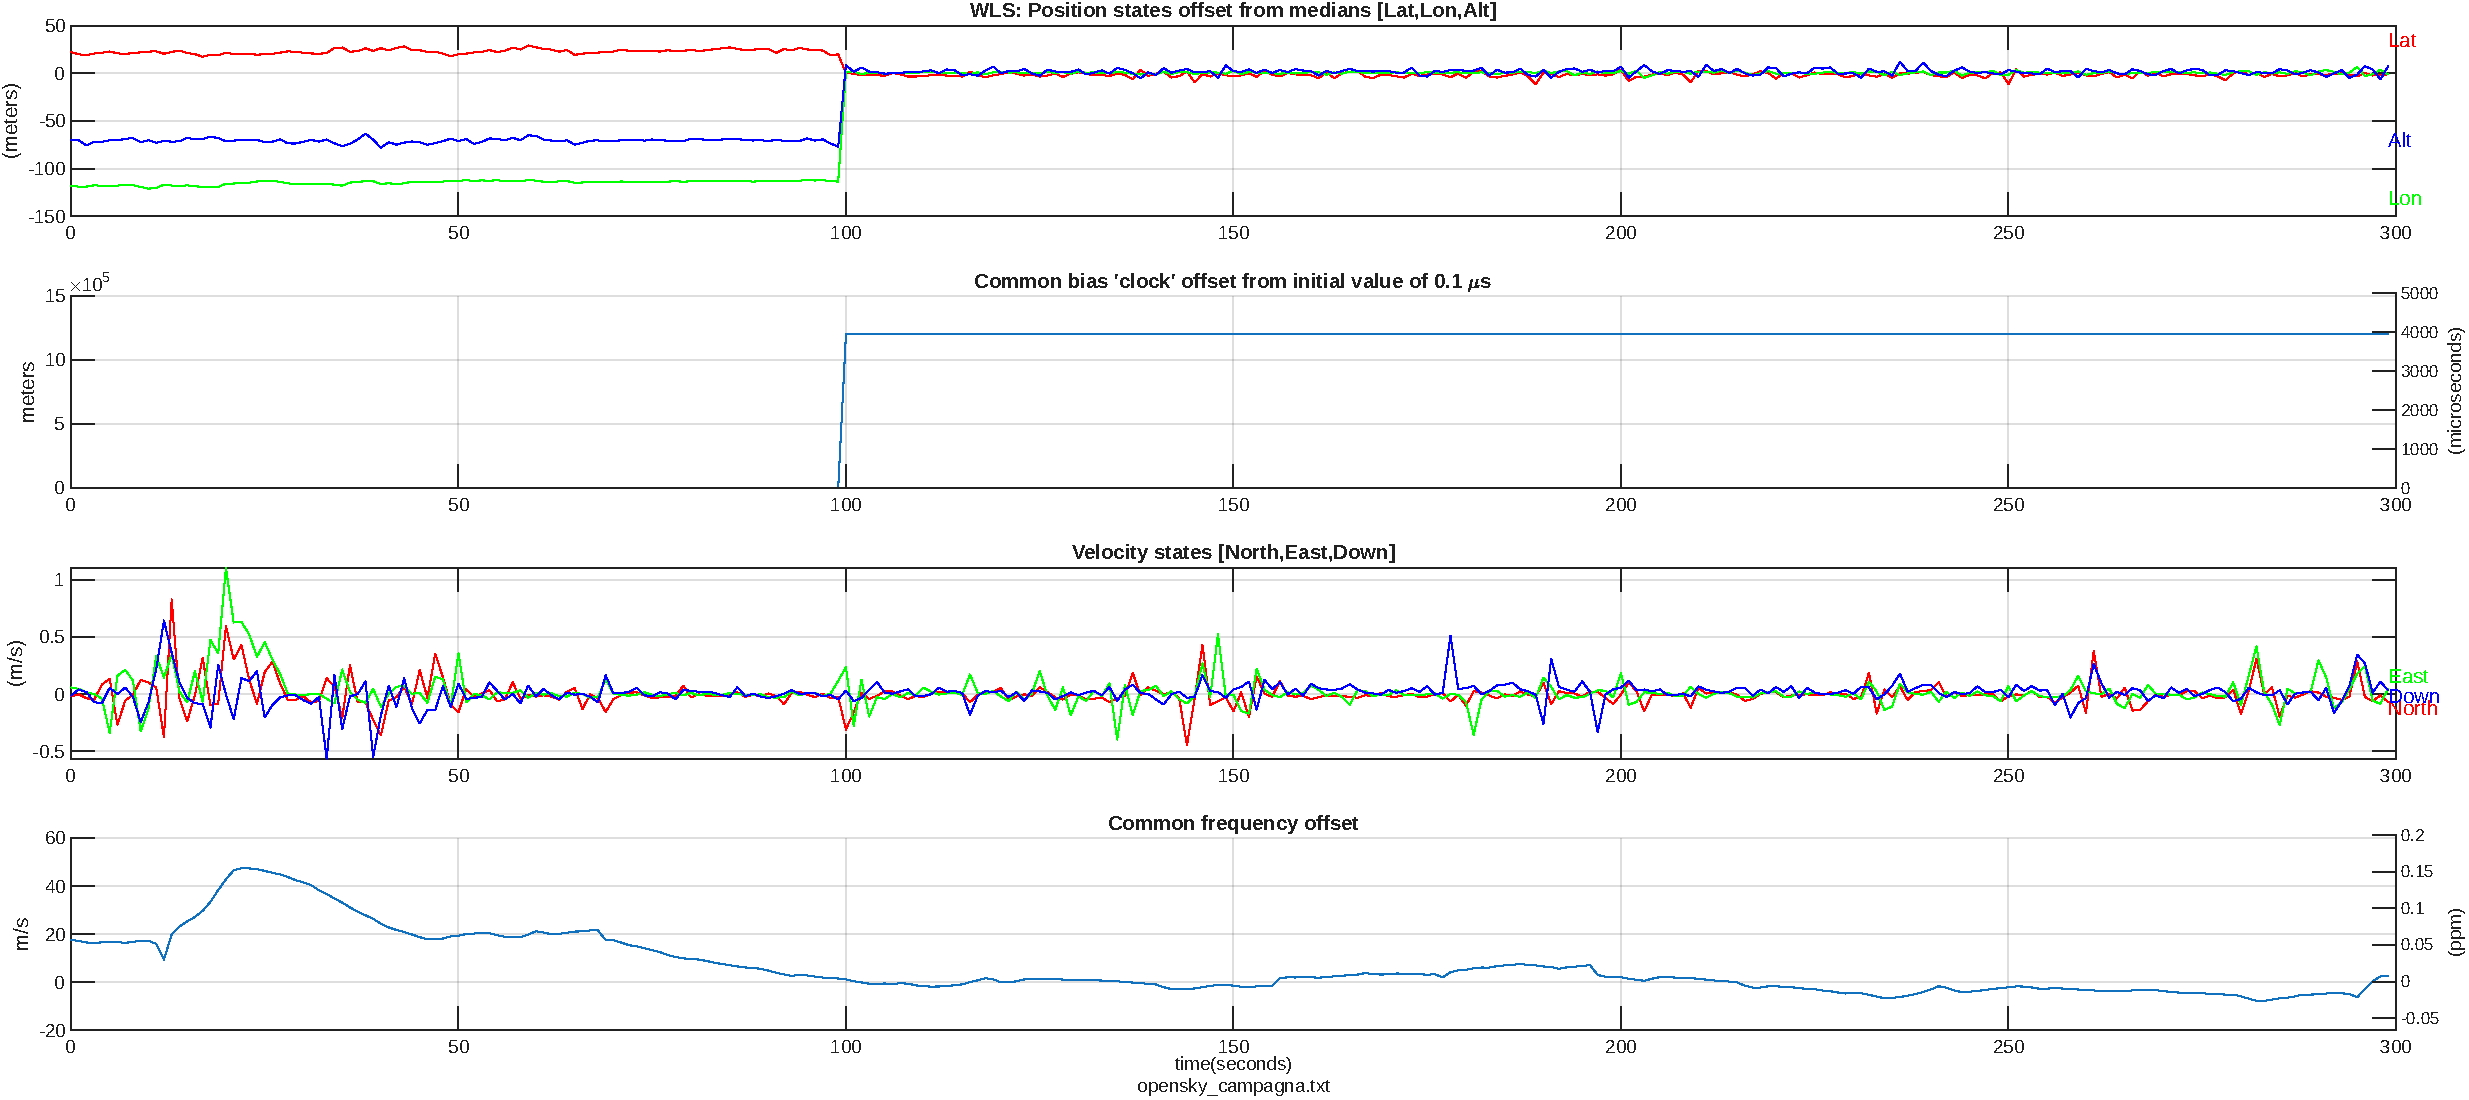
\includegraphics[width=\linewidth]{images/campagna_spoofing_delay/Figure_5.pdf}
        \caption{Position states and Clock bias jump}
        \label{fig:spoof_delay_states}
    \end{subfigure}
    \label{fig:spoof_delay_results}
\end{figure}


\subsection{Position Spoofing far from receiver (with delay)}

Here we executed a harsh spoofing experiment, shifting the target coordinates by approximately 478 km while simultaneously injecting a time delay. This attack represents a worst-case scenario where both the spatial and temporal domains are severely compromised. The "aggressive" spatial translation is evident in the WLS position states (Figure \ref{fig:spoof_torino_diff}): the offsets for latitude, longitude, and altitude immediately jump on the order of $10^5$ meters. Naturally, such an extreme discontinuity generates a completely unphysical and massive anomaly spike in the pseudorange rates. Consequently, the WLS solver is forced to compensate for this artificial propagation delay by forcefully adjusting the receiver's clock. As observed in the previous delayed scenario, the common bias clock violently spikes as shown in Figure \ref{fig:spoof_torino_states}. This specific test unequivocally demonstrates that while a "Far" spoofing attack can successfully teleport the computed position coordinates to a completely different geographic region, it leaves obvious traces across observed metrics.
\begin{figure}[htbp]
    \centering
    % Prima riga
    \begin{subfigure}{0.48\columnwidth}
        \centering
        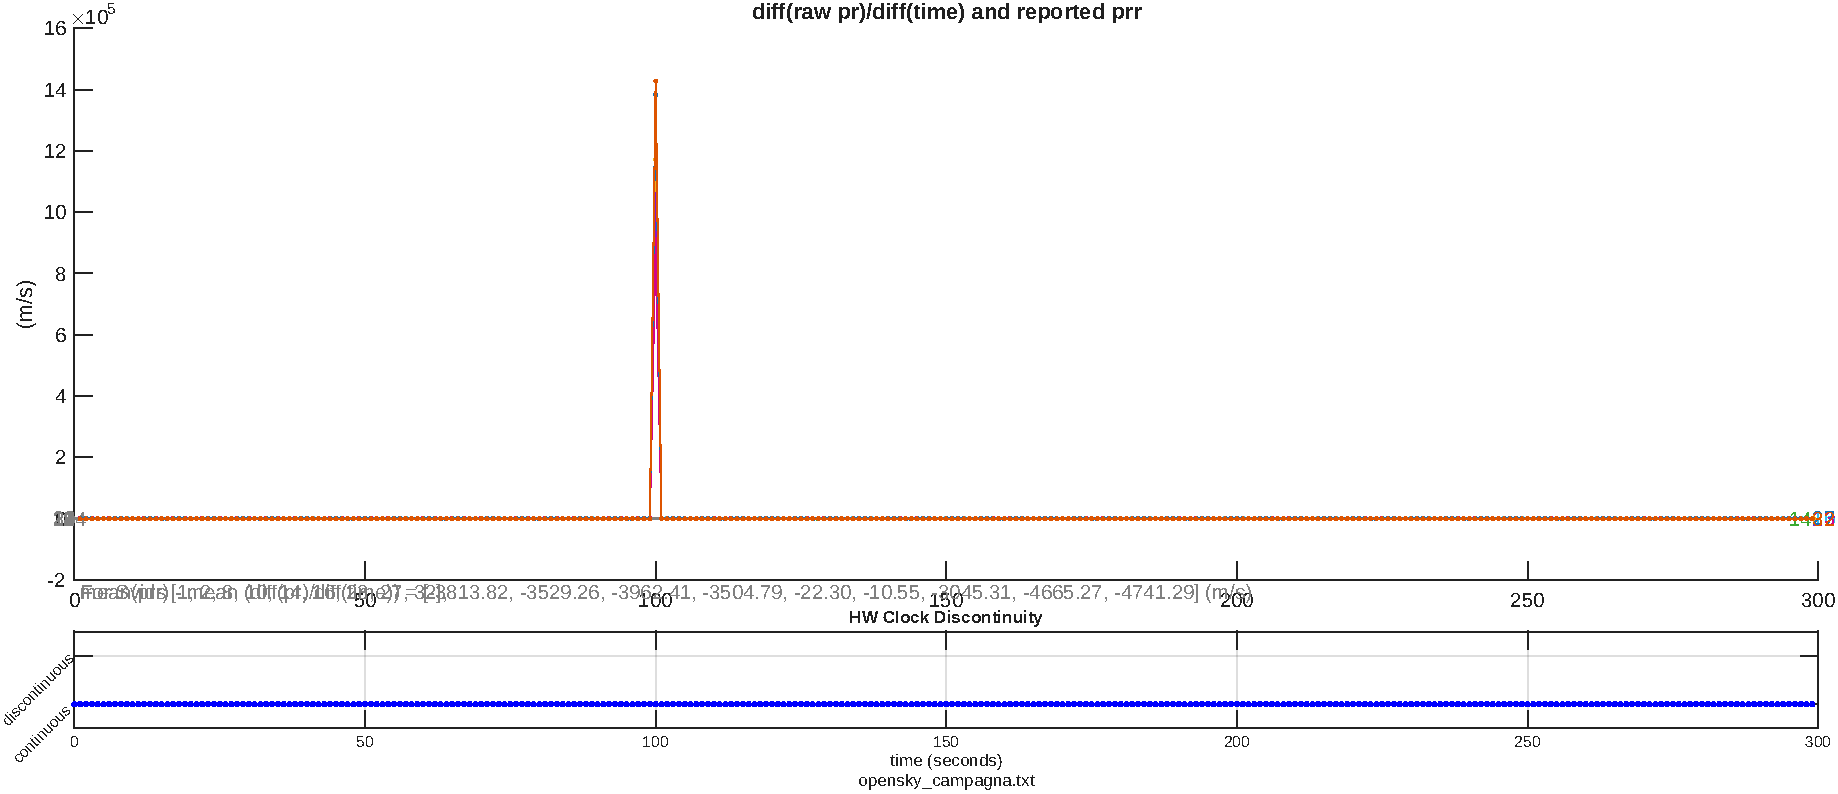
\includegraphics[width=\linewidth]{images/campagna_spoofing_delay_Torino/Figure_2.pdf}
        \caption{Pseudorange rates anomaly}
        \label{fig:spoof_torino_diff}
    \end{subfigure}\hfill
    \begin{subfigure}{0.48\columnwidth}
        \centering
        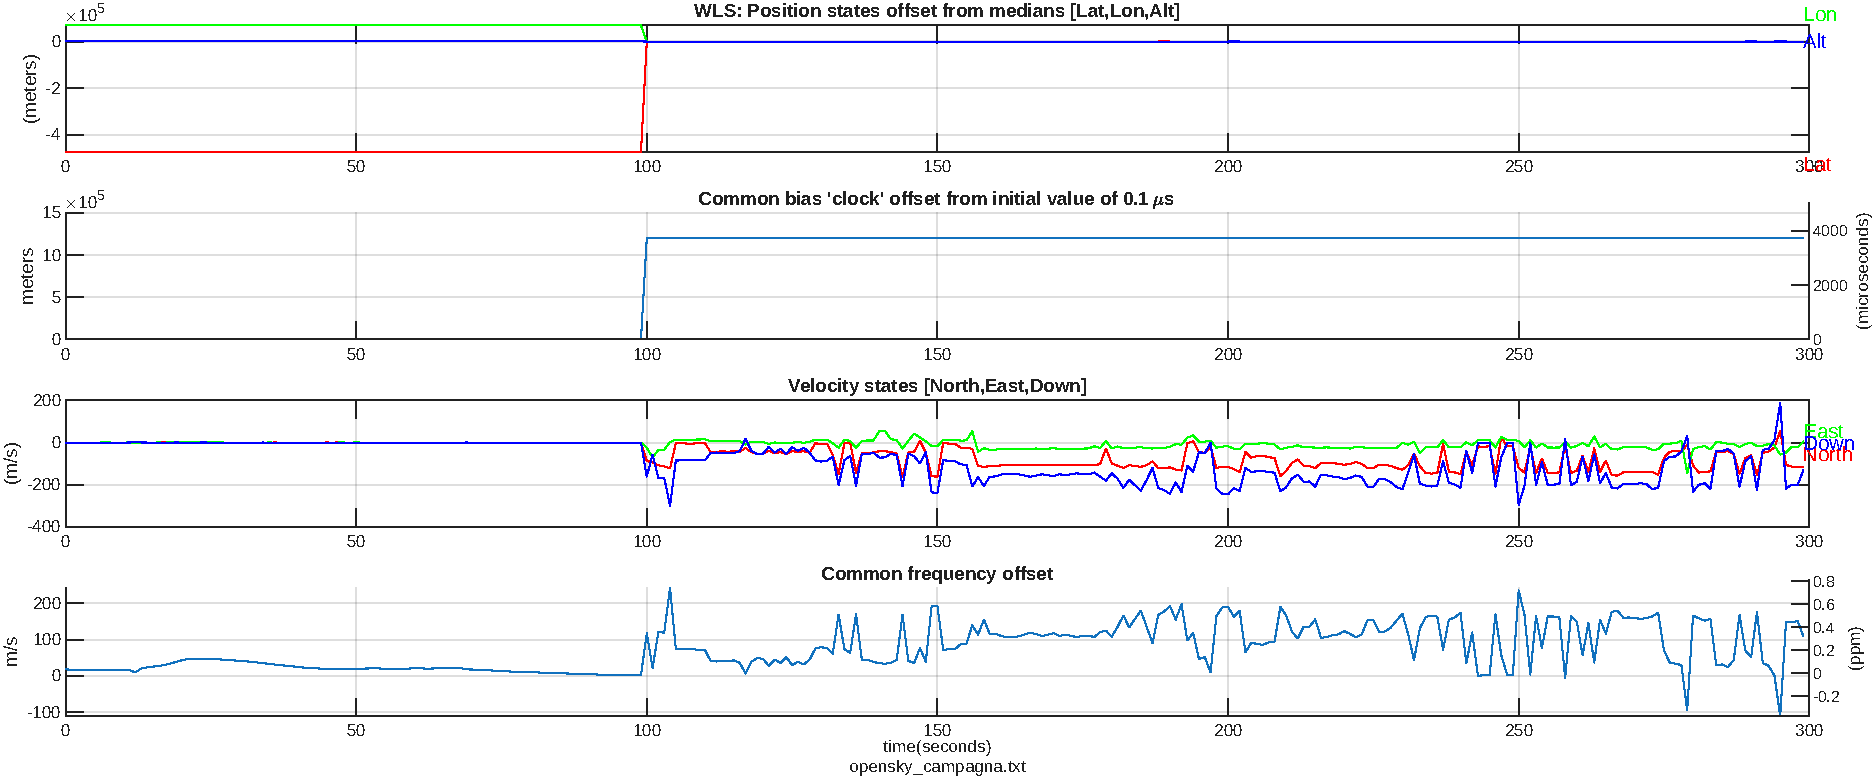
\includegraphics[width=\linewidth]{images/campagna_spoofing_delay_Torino/Figure_5.pdf}
        \caption{Position and Clock bias jump}
        \label{fig:spoof_torino_states}
    \end{subfigure}
\end{figure}


\subsection{Position Spoofing far from receiver (without delay)}

Lastly, we simulated another attack by forcing the coordinates similarly to the previous experiment but with the \texttt{spoof.delay} parameter disabled. The magnitude of the spatial jump forces the WLS solver to register again a violent discontinuity in the position states (Figure \ref{fig:spoof_torino_nodelay_states}), with offsets instantly surging by an order of $10^5$ meters and generating a massive spike in the pseudorange rates. But the most revealing metric here is the receiver's internal clock: since no artificial time delay was introduced, the common bias clock smoothly follows its natural continuous drift. This physical behavior confirms that the WLS solver interpreted the manipulated measurements strictly as an instantaneous spatial teleportation, compromising the position domain while leaving the temporal synchronization intact.
\begin{figure}[htbp]
    \centering
    \begin{subfigure}{0.48\columnwidth}
        \centering
        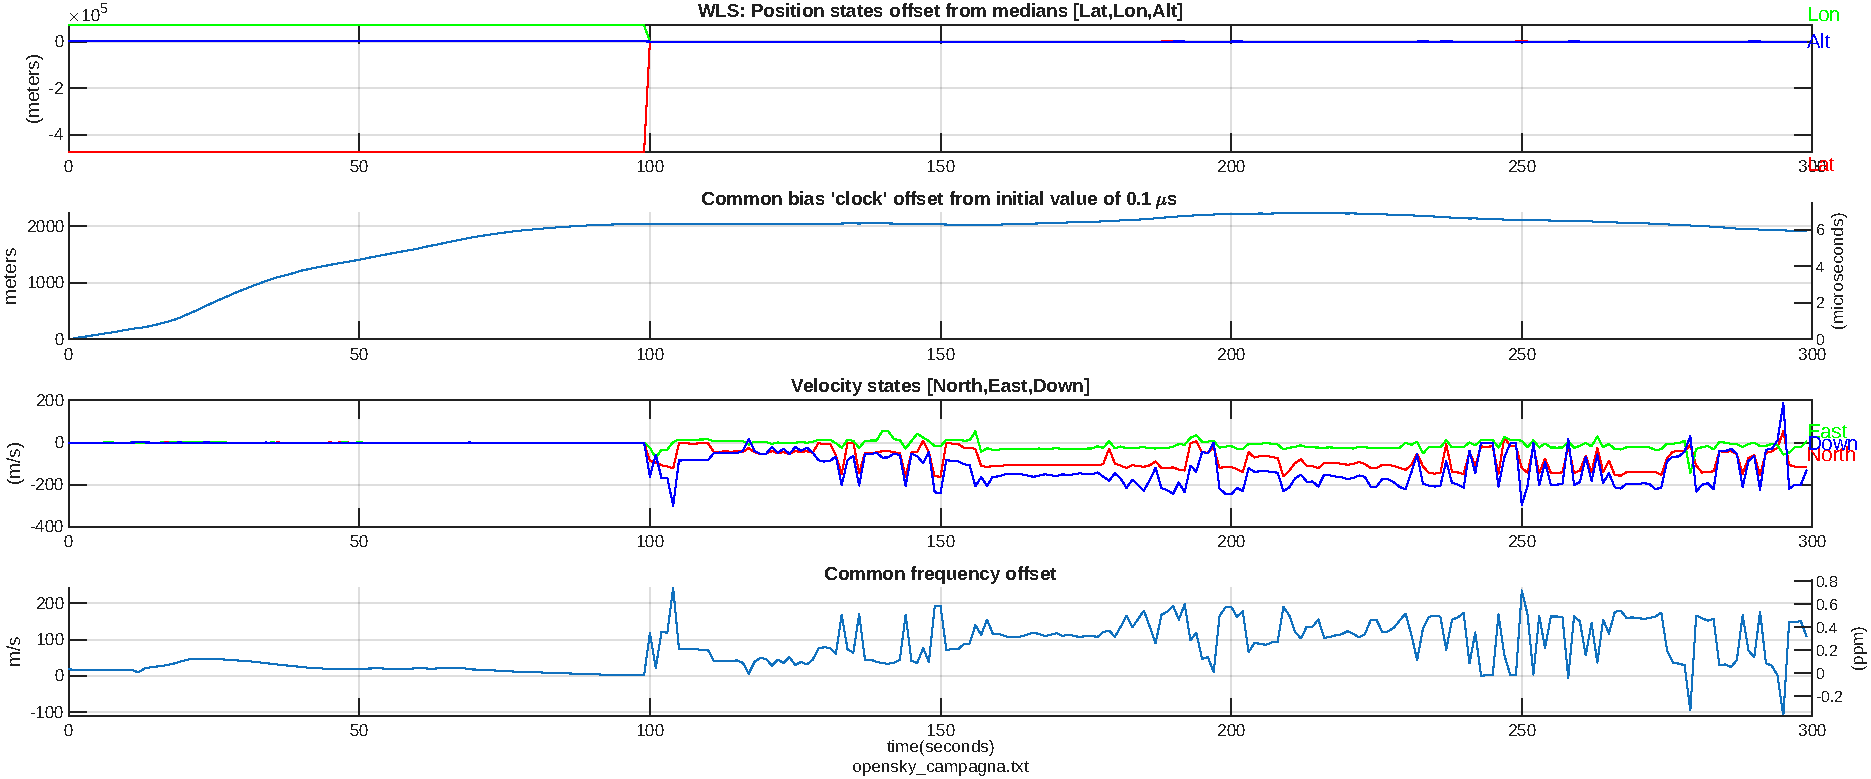
\includegraphics[width=\linewidth]{images/campagna_spoofing_no_delay_Torino/Figure_5.pdf}
        \caption{Position jump of $\times 10^5$ m with continuous clock}
        \label{fig:spoof_torino_nodelay_states}
    \end{subfigure}
    \begin{subfigure}{0.48\columnwidth}
        \centering
        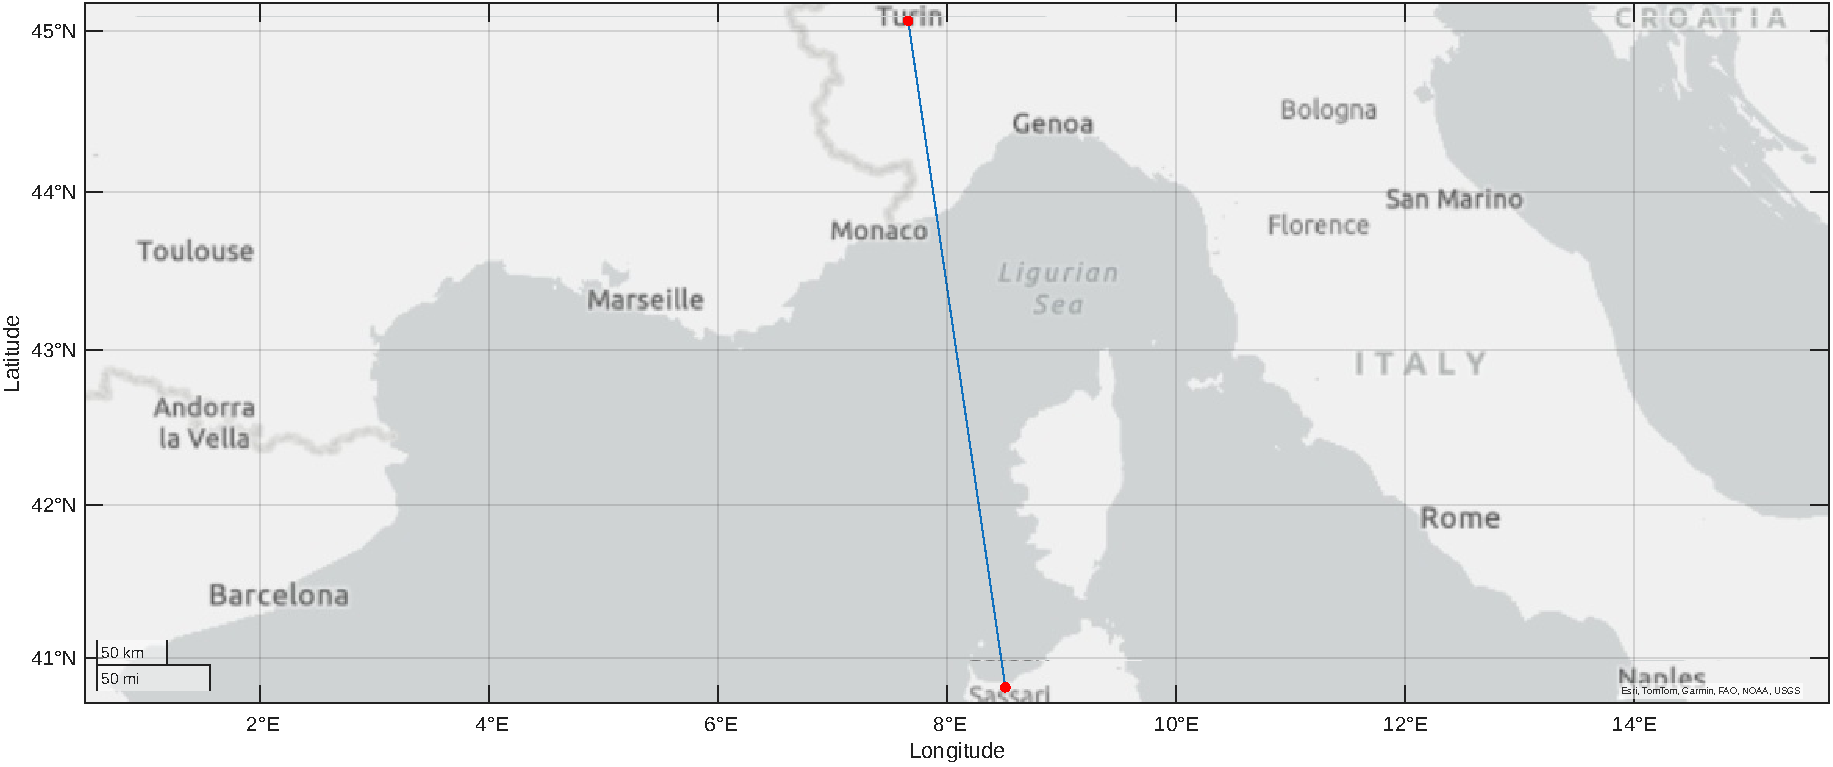
\includegraphics[width=\linewidth]{images/campagna_spoofing_no_delay_Torino/[Optional] Plot Positioning Solution on Map.pdf}
        \caption{Actual location vs physical position}
        \label{fig:spoof_torino_nodelay_position}
    \end{subfigure}
    \label{fig:spoof_torino_nodelay_results}
\end{figure}